% DAFN24 - Robotics - Lecture 8
% Roberto Masocco <roberto.masocco@uniroma2.it>
% June 5, 2024

\documentclass[aspectratio=169]{beamer}

% Slides layout
\usepackage[
    title={Localization and mapping},
    subtitle={From EKF to SLAM},
    event={DAFN},
    author={Roberto Masocco},
    longauthor={Roberto Masocco},
    email={roberto.masocco@uniroma2.it},
    institute={Tor Vergata},
    longinstitute={University of Rome Tor Vergata},
    department={Department of Civil Engineering and Computer Science Engineering},
    researchgroup={},
    date={June 12, 2024}
]{utvengbeamer}

% Code listings settings
\usepackage[nomath]{lmodern}
\definecolor{codegreen}{rgb}{0 0.5 0}
\definecolor{codered}{rgb}{1 0 0}
\definecolor{codeocher}{rgb}{0.8 0.47 0.13}
\usepackage{listings}
\lstdefinestyle{beamer}{
    basicstyle=\ttfamily\small,
    commentstyle=\color{codegreen},
    breakatwhitespace=false,
    captionpos=b,
    frame=lines,
    keepspaces=true,
    keywordstyle=\color{codered}\bfseries,
    numbers=left,
    numbersep=5pt,
    numberstyle=\footnotesize,
    showspaces=false,
    showstringspaces=false,
    showtabs=false,
    stringstyle=\color{codeocher},
    tabsize=2
}
\lstset{style=beamer}
\lstdefinelanguage{Dockerfile}{
  alsoletter={[, ], _, /},
  morecomment=[l][\color{codegreen}]{\#},
  morekeywords={FROM, RUN, ADD, COPY, LABEL, ENV, ARG, CMD}
}
\lstdefinelanguage{compose}{
  alsoletter={:, -, /},
  morecomment=[l][\color{codegreen}]{\#},
  morekeywords={services:, build:, context:, network_mode:, args:, environment:, command:, volumes:, image:, -}
}

\usepackage{multimedia}
\usepackage{hyperref}
\usepackage{wasysym}

\begin{document}

% --- Title page ---
\frame{\titlepage}

% --- Table of contents ---
\begin{frame}
\frametitle{Roadmap}
\tableofcontents
\end{frame}

% --- Section 1 ---
% Section 1 - The perception problem
% Roberto Masocco <roberto.masocco@uniroma2.it>
% June 5, 2024

% ### The perception problem ###
\section{The perception problem}
\graphicspath{{figs/section1/}}

% --- The perception problem ---
\begin{frame}{The perception problem}{Definition}
  To be able to operate autonomously, a robot must continuously answer the following questions:
  \begin{itemize}
    \item \textbg{Where am I?}
    \item \textbg{What is this place?}
  \end{itemize}
  \medskip
  Thus, it must be able to \textbg{perceive} the environment, gathering information useful to:
  \begin{itemize}
    \item \textbg{localize itself}, \emph{i.e.}, continuously estimate its \textbg{pose} as \textbg{both position and orientation} in 3D space;
    \item \textbg{map the environment}, \emph{i.e.}, build a \textbg{representation} of the environment useful to \textbg{navigate} within it.
  \end{itemize}
\end{frame}
\begin{frame}{The perception problem}{Challenges}
  The perception problem is challenging because:
  \begin{itemize}
    \item the environment may be \textbg{partially observable}, \emph{i.e.}, the robot can only perceive a \textbg{subset} of it, and need to update its information in real time;
    \item the environment may be \textbg{dynamic}, \emph{i.e.}, it can change over time;
    \item measurements are always subject to \textbg{noise}.
  \end{itemize}
  \medskip
  The perception problem is usually solved by \textbg{sensor fusion}, \emph{i.e.}, combining information from \textbg{multiple sensors} to obtain a more \textbg{accurate} and \textbg{reliable} estimate of the environment, possibly accounting for \textbg{sensor faults}.
\end{frame}
\begin{frame}{The perception problem}{Tools for the job}
  The tools that robots use to gather \textbg{measurements} from the environment are called \textbg{sensors}.\\
  \medskip
  They can be classified as:
  \begin{itemize}
    \item \textbg{proprioceptive}, \emph{i.e.}, measuring robotic interaction with the environment (\emph{e.g.}, \textbg{encoders}, \textbg{GPS}, \textbg{IMUs});
    \item \textbg{exteroceptive}, \emph{i.e.}, measuring the environment itself (\emph{e.g.}, \textbg{cameras}, \textbg{LiDARs}, \textbg{radars});
    \item \textbg{interoceptive}, \emph{i.e.}, measuring the robot's internal state.
  \end{itemize}
\end{frame}
\begin{frame}{The perception problem}{Tools for the job}
  As any other measurement tool, sensors are based on \textbg{physical principles} and \textbg{energy exchanges}, translating the information they gather into \textbg{electrical signals} that can be acquired and/or processed by a computer.\\
  \medskip
  They are usually characterized by at least:
  \begin{itemize}
    \item a \textbg{digital} or \textbg{analog} \textbg{encoding} of the measurement;
    \item a \textbg{frame of reference} in which the measurement is expressed;
    \item \textbg{accuracy} and \textbg{uncertainty} parameters.
  \end{itemize}
\end{frame}
\begin{frame}{The perception problem}{Tools for the job}
  \begin{figure}
    \centering
    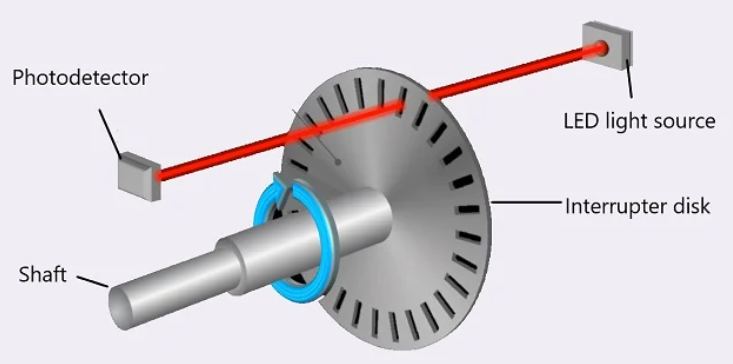
\includegraphics[width=.75\textwidth]{encoder.png}
    \caption{Rotary encoder working principle.}
    \label{fig:encoder}
  \end{figure}
\end{frame}
\begin{frame}{The perception problem}{Tools for the job}
  \begin{figure}
    \centering
    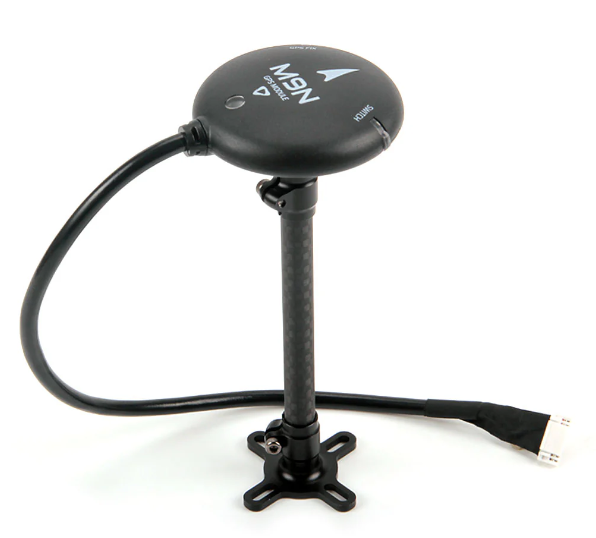
\includegraphics[width=.4\textwidth]{gps}
    \caption{GPS module for drones.}
    \label{fig:gps}
  \end{figure}
\end{frame}
\begin{frame}{The perception problem}{Tools for the job}
  \begin{figure}
    \centering
    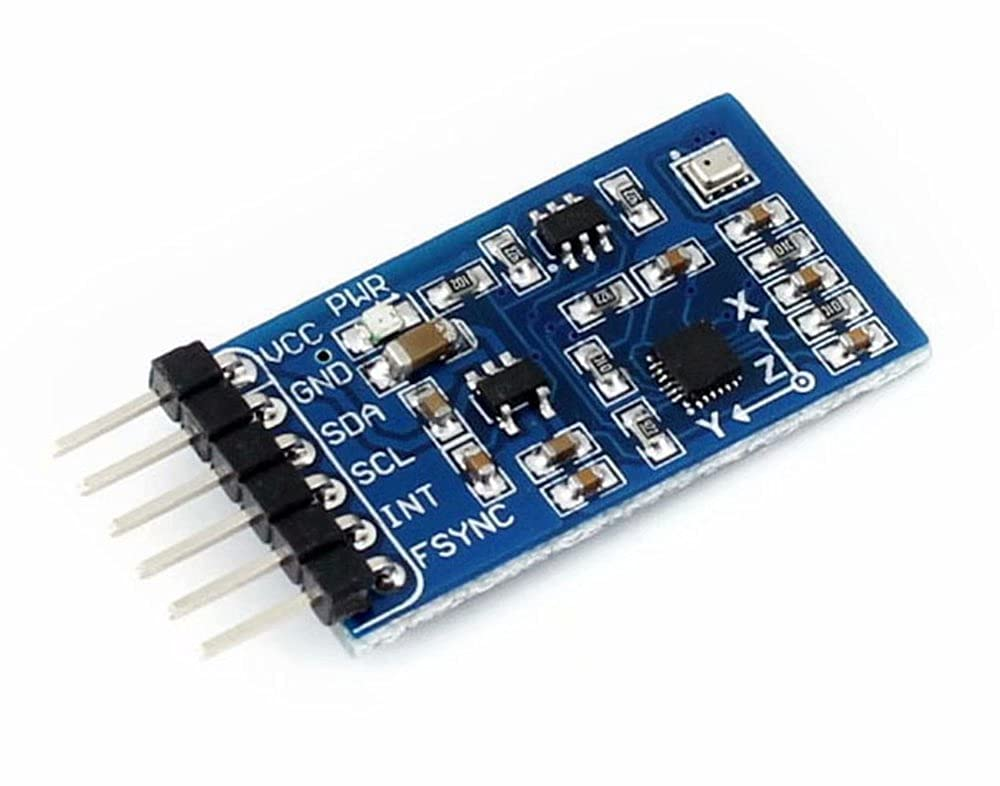
\includegraphics[width=.45\textwidth]{imu}
    \caption{Inertial Measurement Unit (IMU).}
    \label{fig:imu}
  \end{figure}
\end{frame}
\begin{frame}{The perception problem}{Tools for the job}
  \begin{figure}
    \centering
    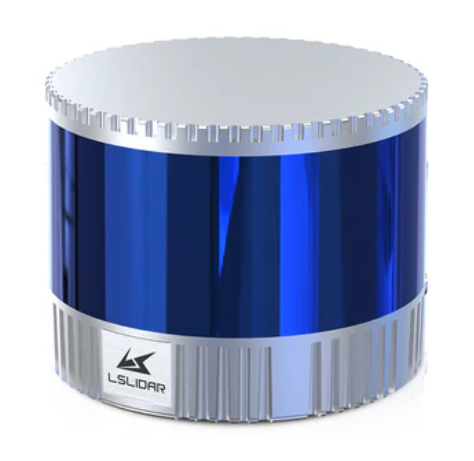
\includegraphics[width=.38\textwidth]{lidar}
    \caption{Light Detection and Ranging (LiDAR) sensor.}
    \label{fig:lidar}
  \end{figure}
\end{frame}
\begin{frame}{The perception problem}{Tools for the job}
  \begin{figure}
    \centering
    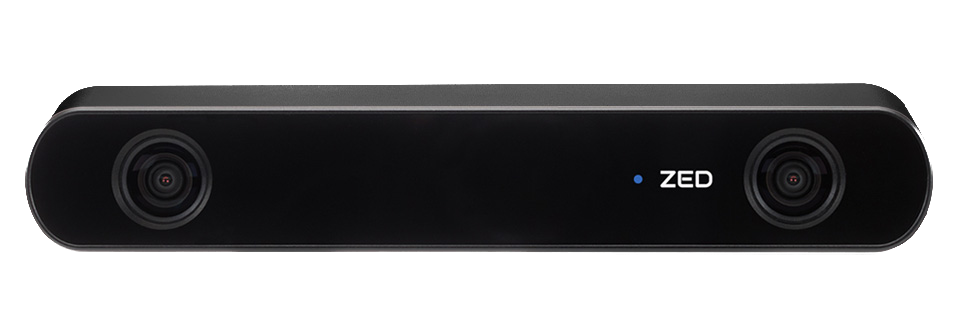
\includegraphics[width=.8\textwidth]{zed2i}
    \caption{ZED 2i stereo camera.}
    \label{fig:zed2i}
  \end{figure}
\end{frame}


% --- Section 2 ---
% Section 2 - Common interfaces
% Roberto Masocco <roberto.masocco@uniroma2.it>
% June 5, 2024

% ### Common interfaces ###
\section{Common interfaces}

% --- Common interfaces ---
\begin{frame}{Common interfaces}
	A standard ROS 2 installation offers many \textbg{interface packages} (\emph{i.e.}, messages), to provide \textbg{standard data types} to communicate sensor measurements and related data.\\
	\bigskip
	The most important are:
	\begin{itemize}
		\item \texttt{sensor\_msgs}, for \textbg{sensor measurements};
		\item \texttt{geometry\_msgs}, for \textbg{geometric data};
		\item \texttt{nav\_msgs}, for \textbg{navigation data}.
	\end{itemize}
	\medskip
	It is suggested to \textbg{always use these message types}, plus common best practices, to ensure full interoperability between sensor drivers and localization and mapping algorithms.\\
  \bigskip
  Try to \texttt{ros2 interface show} these messages to understand their structure!
\end{frame}

% --- sensor_msgs ---
\begin{frame}{\texttt{sensor\_msgs}}{Common interfaces for sensors}
	\begin{itemize}
		\item \texttt{Imu}
		\item \texttt{JointState}
		\item \texttt{CameraInfo} and \texttt{Image}
		\item \texttt{LaserScan}
		\item \texttt{PointCloud2}
		\item \texttt{Temperature}
		\item \texttt{NavSatFix}
		\item \texttt{Illuminance}
		\item ...
	\end{itemize}
\end{frame}

% --- geometry_msgs ---
\begin{frame}{\texttt{geometry\_msgs}}{Common interfaces for algebraic data}
  \begin{itemize}
    \item \texttt{Vector3Stamped}
    \item \texttt{QuaternionStamped}
    \item \texttt{PoseWithCovarianceStamped}
    \item \texttt{TwistWithCovarianceStamped}
    \item \texttt{TransformStamped} (used by tf2!)
    \item \texttt{AccelWithCovarianceStamped}
    \item ...
  \end{itemize}
\end{frame}

% --- nav_msgs ---
\begin{frame}{\texttt{nav\_msgs}}{Common interfaces for navigation data}
  \begin{itemize}
    \item \texttt{Odometry} (\texttt{Header}, body (child) frame ID, \texttt{PoseWithCovariance}, \texttt{TwistWithCovariance})
    \item \texttt{Path}
    \item \texttt{OccupancyGrid}
    \item ...
  \end{itemize}
\end{frame}


% --- Section 3 ---
% Section 3 - The tf2 library
% Roberto Masocco <roberto.masocco@uniroma2.it>
% June 5, 2024

% ### The tf2 library ###
\section{The tf2 library}
\graphicspath{{figs/section5/}}

% --- Rigid transformations ---
\begin{frame}{Rigid transformations}
	When a robot moves in space, it is important to keep track of its \textbg{position} and \textbg{orientation} with respect to a \textbg{reference frame}.\\
	\bigskip
	Sensors measuring this information, as well as many more, are \textbg{mounted} on the robot, in fixed positions and orientations.\\
	\bigskip
	To process these measurements, they must first be \textbg{transformed} from the \textbg{body frame} into a common reference frame, usually called:
	\begin{itemize}
		\item \textbg{world frame} (world origin), in the case of \textbg{global localization};
		\item \textbg{local frame}, or \textbg{odom frame} (robot starting point), in the case of \textbg{local localization}.
	\end{itemize}
	\medskip
	Such \textbg{rigid transformations} are \textbg{isometries}. They must be applied to almost every sensor measurement, and are usually \textbg{composable}.\\
	\bigskip
	We would like the middleware to provide tools to do this almost automatically...
\end{frame}

% --- The tf2 library ---
\begin{frame}{The tf2 library}
	\begin{columns}
		\column{.6\textwidth}
		\texttt{tf2} is the \textbg{standard ROS 2 library} to handle rigid transformations. It allows to:
		\begin{itemize}
			\item \href{https://docs.ros.org/en/humble/Tutorials/Intermediate/Tf2/Writing-A-Tf2-Broadcaster-Cpp.html}{\color{blue}\underline{\textbf{broadcast}}} and \href{https://docs.ros.org/en/humble/Tutorials/Intermediate/Tf2/Writing-A-Tf2-Listener-Cpp.html}{\color{blue}\underline{\textbf{listen}}} to transformations;
			\item optimize the broadcasting of \textbg{static transformations} vs the buffering of the others;
			\item \textbg{transform} any kind of sensor data from one frame to another, making efficient computations in C++ code relying on the \texttt{Eigen} mathematical library;
			\item broadcast static \textbg{robot descriptions} from \texttt{URDF} files, listing links and joints and how they are connected, resulting in a \textbg{tree-like structure};
			\item \textbg{command-line tools} to introspect the tf tree.
		\end{itemize}

		\column{.4\textwidth}
		\begin{figure}
			\centering
			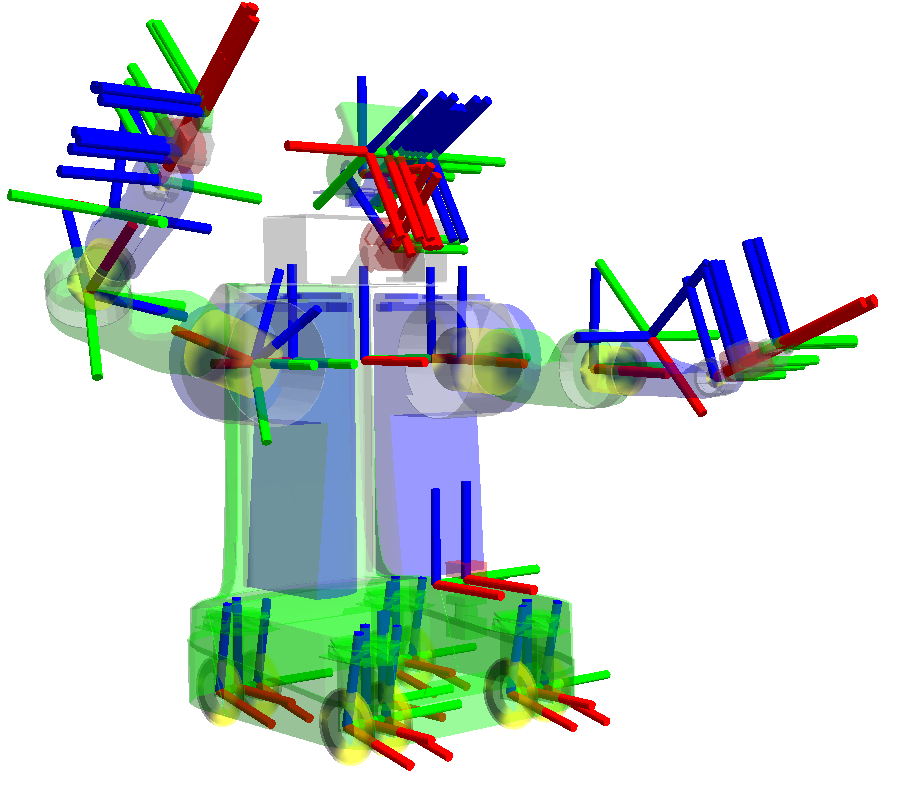
\includegraphics[width=.9\textwidth]{ros2_tf2}
			\caption{Example of robot description with tf2.}
			\label{fig:tf2example}
		\end{figure}
	\end{columns}
\end{frame}
\begin{frame}{The tf2 library}
	\begin{figure}
		\centering
		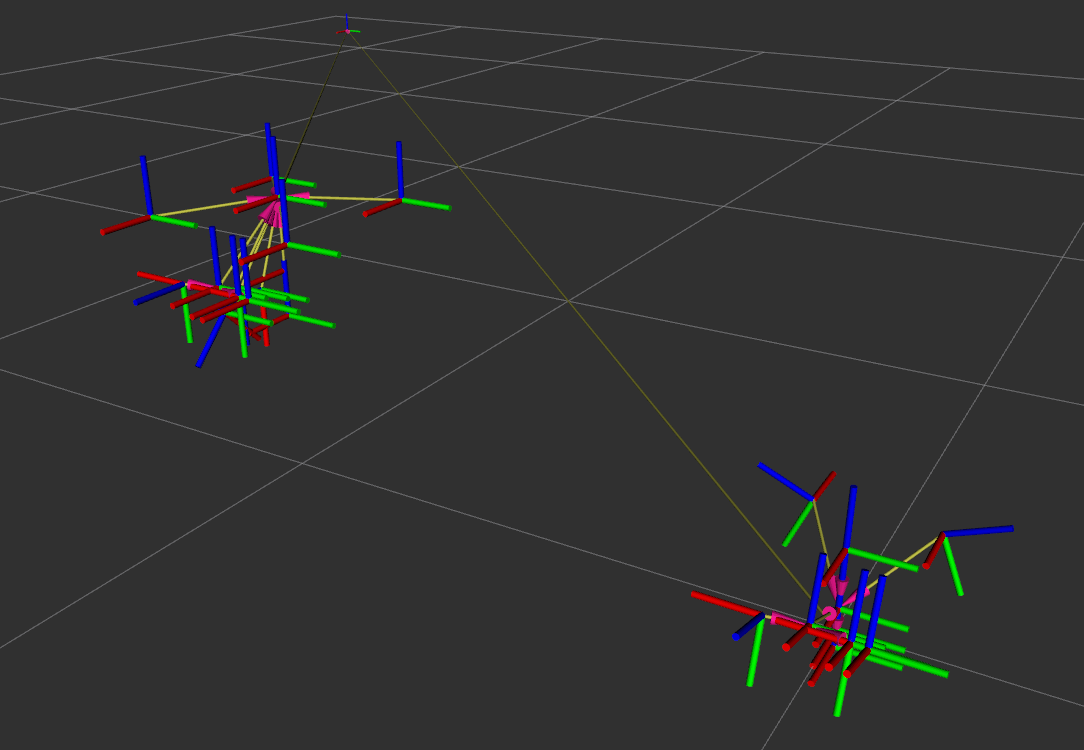
\includegraphics[width=.58\textwidth]{tfs}
		\caption{Broadcasted robot descriptions, plus real-time transformations given by localization systems.}
		\label{fig:tfs}
	\end{figure}
\end{frame}


% --- Section 4 ---
% Section 4 - The Extended Kalman Filter
% Roberto Masocco <roberto.masocco@uniroma2.it>
% June 7, 2024

% ### The Extended Kalman Filter ###
\section{The Extended Kalman Filter}

% --- Odometric reconstruction ---
\begin{frame}{Odometric reconstruction}{An elementary sensor fusion technique}
  \visible<1->{
    Suppose you have a robot equipped with $m$ \textbg{sensors} producing \textbg{measurements} $q_i$, $i = 1,\dotsc,m$, and a \textbg{motion model} that predicts the \textbg{state} of the robot $x_k$ at time $k$ given the state $x_{k-1}$ at time $k-1$ and the control input $u_k$ applied to the robot.\\
    \bigskip
    You can use these data to perform an \textbg{odometric reconstruction}: integrating the motion model with sensor data and the \textbg{estimated state} of the robot.
  }
  \visible<2>{
    \bigskip
    \begin{alertblock}{}
      \centering
      \textbr{Measurements are affected by noise, that this technique does not account for.}
    \end{alertblock}
    Noise may even be due to \textbg{physical phenomena} like slippage, vibrations, or sensor faults.
  }
\end{frame}

% --- Modelling noise ---
\begin{frame}{Modelling noise}{Gaussian random variables}
  Suppose that $m=2$. At any given time, the \textbg{measurement} of a quantity $x$ can be modeled as a \textbg{Gaussian random variable} centered around the \textbg{true value} of $x$ with a certain \textbg{standard deviation}:
  \begin{itemize}
    \item $q_1 \sim \mathcal{N}(x,\sigma_1^2)\,$;
    \item $q_2 \sim \mathcal{N}(x,\sigma_2^2)\,$.
  \end{itemize}
  Having distinct sensors makes these variables \textbg{independent}.\\
  These assumptions are reasonable because:
  \begin{itemize}
    \item of well-known results, \emph{e.g.}, the Central Limit Theorem;
    \item the \textbg{average} is the real value of $x$ if we rule out \textbg{systematic errors} by, \emph{e.g.}, calibrating the sensor;
    \item the \textbg{variance} models the \textbg{dispersion} of the measurements around the central value.
  \end{itemize}
\end{frame}
\begin{frame}{Modelling noise}{Gaussian random variables}
  Note that, by relying on \textbg{independence}, \textbg{Bayes' theorem}, and the \textbg{properties} of the Gaussian distribution:
  \begin{itemize}
    \item $q_1 \sim \mathcal{N}(x,\sigma_1^2) \Rightarrow x \sim \mathcal{N}(q_1,\sigma_1^2)\,$;
    \item $q_2 \sim \mathcal{N}(x,\sigma_2^2) \Rightarrow x \sim \mathcal{N}(q_2,\sigma_2^2)\,$;
  \end{itemize}
  \emph{i.e.}, $x$ \textbg{is also a Gaussian random variable} centered around a measurement.
\end{frame}
\begin{frame}{Modelling noise}{Combining variables}
  \textbg{A priori}, and in particular before getting any measurements, we can \textbg{assume that $x$ has a uniform distribution}, making $p(x)$ \textbg{independent} from both $p(q_1)$ and $p(q_2)$.\\
  \bigskip
  Relying on the same previous results, we can \textbg{combine the two measurements} $q_1$ and $q_2$ to obtain a \textbg{better estimate} of $x$, as $x \sim \mathcal{N}(q,\sigma^2)$, where:
  \begin{itemize}
    \item $q = \frac{\sigma_2^2 q_1 + \sigma_1^2 q_2}{\sigma_1^2 + \sigma_2^2}\,$;
    \item $\sigma^2 = \frac{\sigma_1^2 \sigma_2^2}{\sigma_1^2 + \sigma_2^2}\,$;
  \end{itemize}
  \emph{i.e.}, $x$ is a new Gaussian random variable centered around a \textbg{weighted average} of the measurements, with a \textbg{variance} that decreases as the \textbg{uncertainty} of the measurements decreases.
\end{frame}
\begin{frame}{Modelling noise}{Combining variables}
  To see this, start from using \textbg{independence} to see what it means to get $q_1$ and $q_2$:
  \begin{equation*}
    p((q_1,q_2)|x) = p(q_1|x)p(q_2|x) = \dotsc = \eta e^{-\frac{(x-q)^2}{2\sigma^2}}\,,
  \end{equation*}
  where
  \begin{equation*}
    \eta = \frac{1}{2\pi\sigma_1\sigma_2} e^{\frac{q^2}{2\sigma^2} - \frac{q_1^2}{2\sigma_1^2} - \frac{q_2^2}{2\sigma_2^2}}\,.
  \end{equation*}
  Then, \textbg{Bayes} tells you that
  \begin{equation*}
    p(x|(q_1,q_2)) = p((q_1,q_2)|x)\frac{p(x)}{p((q_1,q_2))} = \frac{\eta p(x)}{p((q_1,q_2))} e^{-\frac{(x-q)^2}{2\sigma^2}} = \tilde{\eta} e^{-\frac{(x-q)^2}{2\sigma^2}}\,,
  \end{equation*}
  where $\tilde{\eta}$ is constant due to all the hypotheses made, and in particular
  \begin{equation*}
    \int_{-\infty}^{+\infty} p(x|(q_1,q_2))dx = 1 \implies \tilde{\eta} = \frac{1}{\sqrt{2\pi\sigma^2}}\,.
  \end{equation*}
\end{frame}

% --- Combining two measurements ---
\begin{frame}{Combining two measurements}{Step by step}
  Suppose you have to update an \textbg{estimate} $\hat{x}$ of a quantity $x$ and its \textbg{variance} $\Sigma^2$ with two measurements $q_1$ and $q_2$:
  \begin{enumerate}
    \item Measurement $q_1$ arrives: $\hat{x}_1 = q_1$, $\Sigma_1^2=\sigma_1^2$.
    \item Measurement $q_2$ arrives.
    \item $\hat{x}_{1,2} = \frac{\Sigma_1^2 q_2 + \sigma_2^2 \hat{x}_1}{\Sigma_1^2 + \sigma_2^2} = \hat{x}_1 + \frac{\Sigma_1^2}{\Sigma_1^2+\sigma_2^2}(q_2 - \hat{x}_1)\,$.
    \item $\Sigma_{1,2}^2 = \frac{\Sigma_1^2 \sigma_2^2}{\Sigma_1^2 + \sigma_2^2} = (1-\frac{\Sigma_1^2}{\Sigma_1^2+\sigma_2^2})\Sigma_1^2\,$.
  \end{enumerate}
\end{frame}

% --- Combining many measurements ---
\begin{frame}{Combining many measurements}{The first innovation}
  Suppose now that you can receive $m$ measurements in \textbg{subsequent steps}. Then:
  \begin{equation}
    \hat{x}_{k+1} = \hat{x}_k + V_{k+1}(q_{k+1} - \hat{x}_k)\,,
  \end{equation}
  \begin{equation}
    \Sigma_{k+1}^2 = (1 - V_{k+1})\Sigma_k^2\,,
  \end{equation}
  where:
  \begin{equation}
    V_{k+1} = \frac{\Sigma_k^2}{\Sigma_k^2 + \sigma_{k+1}^2}\,,
  \end{equation}
  and $V_{k+1} \in (0,1)$. It is a \textbg{sampled approximation}.\\
  Note what happens when the new $k+1$-th measurement is either \textbg{very accurate} ($\sigma_{k+1}^2 \ll \Sigma_k^2$) or \textbg{very noisy} ($\sigma_{k+1}^2 \gg \Sigma_k^2$).
\end{frame}

% --- Kalman filter ---
\begin{frame}{Kalman filter}{The scalar case}
  Suppose you have a \textbg{dynamic system} with a \textbg{discrete-time model}:
  \begin{equation}
    x_{k+1} = ax_k + bu_k + \omega_k\,,
  \end{equation}
  with $\omega_k \sim \mathcal{N}(0,\sigma_{\omega}^2)$, and \textbg{measurements that depend on the state}:
  \begin{equation}
    z_k = cx_k + \nu_k\,,
  \end{equation}
  where $\nu_k \sim \mathcal{N}(0,\sigma_{\nu}^2)$ is the \textbg{noise}.
\end{frame}
\begin{frame}{Kalman filter}{The scalar case}
  Initialize the \textbg{estimate} as $\hat{x}_0$ ($0$ is mostly fine) and the \textbg{covariance} as $P_0$ (a rough estimate of the uncertainty).\\
  Then, relying on the same properties as the previous cases:
  \begin{subequations}
    \begin{align}
      \hat{x}_{k+1}^{-} &= a\hat{x}_k + bu_k\,,\label{eq:predictionx}\\
      P_{k+1}^{-} &= a^2P_k + \sigma_{\omega}^2\,,\label{eq:predictioncov}\\
      K_{k+1} &= \frac{P_{k+1}^{-}c}{c^2P_{k+1}^{-} + \sigma_{\nu}^2}\,,\label{eq:kalmangain}\\
      \hat{x}_{k+1} &= \hat{x}_{k+1}^{-} + K_{k+1}(z_{k+1} - c\hat{x}_{k+1}^{-})\,,\label{eq:innovx}\\
      P_{k+1} &= (1 - K_{k+1}c)P_{k+1}\,.\label{eq:innovcov}
    \end{align}
  \end{subequations}
  \eqref{eq:predictionx}-\eqref{eq:predictioncov} compose the \textbg{prediction step} of the \textbg{a priori estimate}, \eqref{eq:kalmangain} is the \textbg{Kalman gain}, and \eqref{eq:innovx}-\eqref{eq:innovcov} are the \textbg{correction step}, applying the \textbg{innovation term} to compute the \textbg{a posteriori estimate}.
\end{frame}
\begin{frame}{Kalman filter}{The vectorial case}
  The \textbg{vectorial case} is a \textbg{generalization} of the scalar case, using \textbg{vectors} and \textbg{covariance matrices}.\\
  Suppose that now you have this model:
  \begin{equation}
    x_{k+1} = Ax_k + Bu_k + \omega_k\,,
  \end{equation}
  where $A$ and $B$ are \textbg{matrices}, $\omega_k \sim \mathcal{N}(0,Q_{\omega})$, and the \textbg{measurement} is:
  \begin{equation}
    z_k = Cx_k + \nu_k\,,
  \end{equation}
  where $\nu_k \sim \mathcal{N}(0,Q_{\nu})$.\\
  $Q_\omega$, $Q_\nu$ are the \textbg{covariance matrices} of the noises: this notation assumes that they are \textbg{constant} but in case they are \textbg{time-varying}, the following would work in the same way.
\end{frame}
\begin{frame}{Kalman filter}{The vectorial case}
  By applying the same reasoning as before, with appropriate algebraic manipulations:
  \begin{subequations}
    \begin{align}
      \hat{x}_{k+1}^{-} &= A\hat{x}_k + Bu_k\,,\label{eq:predictionxvec}\\
      P_{k+1}^{-} &= AP_kA^T + Q_{\omega}\,,\label{eq:predictioncovvec}\\
      K_{k+1} &= P_{k+1}^{-}C^T(CP_{k+1}^{-}C^T + Q_{\nu})^{-1}\,,\label{eq:kalmangainvec}\\
      \hat{x}_{k+1} &= \hat{x}_{k+1}^{-} + K_{k+1}(z_{k+1} - C\hat{x}_{k+1}^{-})\,,\label{eq:innovxvec}\\
      P_{k+1} &= (I - K_{k+1}C)P_{k+1}^{-}\,,\label{eq:innovcovvec}
    \end{align}
  \end{subequations}
  where $I$ is the identity matrix.\\
  The idea behind this is still the \textbg{combination of Gaussian random variables}.
\end{frame}

% --- Extended Kalman Filter ---
\begin{frame}{Extended Kalman Filter}{The nonlinear case}
  Suppose you have a \textbg{nonlinear model}:
  \begin{subequations}
    \begin{align}
      x_{k+1} &= f(x_k,u_k,\omega_k)\,,\\
      z_k &= h(x_k,\nu_k)\,,
    \end{align}
  \end{subequations}
  with noises as random variables as before.\\
  In this case, we can resort to a \textbg{linearization} to \textbg{reapply the same reasoning}, but we lose \textbg{convergence properties}.\\
  Nonetheless, the \textbg{Extended Kalman Filter} (EKF) is a \textbg{widely used} heuristic state estimation technique, achieving \textbg{good results} in many practical scenarios.
\end{frame}
\begin{frame}{Extended Kalman Filter}{The linearization}
  Consider two subsequent time instants $k$ and $k+1$.\\
  Given the \textbg{current estimate} $\hat{x}_k$ at time $k$ and the \textbg{prediction} $\hat{x}_{k+1}^{-}$ at time $k+1$, we can write:
  \begin{subequations}
    \begin{align}
      f(x_k,u_k,\omega_k) &= {\color{red}f(\hat{x}_k,u_k,0)} + {\color{red}F_k}(x_k - {\color{red}\hat{x}_k}) + W_k\omega_k + o(\|x_k - \hat{x}_k\|)\,,\label{eq:flin}\\
      h(x_{k+1},\nu_{k+1}) &= {\color{blue}h(\hat{x}_{k+1}^{-},0)} + {\color{blue}H_{k+1}}(x_{k+1} {\color{blue}- \hat{x}_{k+1}^{-}}) + L_{k+1}\nu_{k+1} + o(\|x_{k+1} - \hat{x}_{k+1}^{-}\|)\,,\label{eq:hlin}
    \end{align}
  \end{subequations}
  where $F=\partial f/\partial x$, $W=\partial f/\partial \omega$, $H=\partial h/\partial x$, and $L=\partial h/\partial \nu$ are Jacobian matrices, which we evaluate at appropriate times.\\
  Taking \eqref{eq:flin}-\eqref{eq:hlin} as exact and rearranging known terms, these lead to:
  \begin{subequations}
    \begin{align}
      x_{k+1} &= F_k x_k + {\color{red}f_0(\hat{x}_k,u_k)} + W_k\omega_k\,,\\
      z_{k+1} &= H_{k+1}x_{k+1} + {\color{blue}h_0(\hat{x}_{k+1}^{-})} + L_{k+1}\nu_{k+1}\,,\label{eq:newmeas}
    \end{align}
  \end{subequations}
  which is easier to manage, both in terms of algebra and \textbg{computational complexity}.
\end{frame}
\begin{frame}{Extended Kalman Filter}{The equations}
  By applying the same reasoning as before, with appropriate algebraic manipulations:
  \begin{subequations}
    \begin{align}
      \hat{x}_{k+1}^{-} &= f(\hat{x}_k,u_k,0)\,,\\
      P_{k+1}^{-} &= F_kP_kF_k^T + W_kQ_{\omega}W_k^T\,,\\
      K_{k+1} &= P_{k+1}^{-}H_{k+1}^T(H_{k+1}P_{k+1}^{-}H_{k+1}^T + L_{k+1}Q_{\nu}L_{k+1}^T)^{-1}\,,\\
      \hat{x}_{k+1} &= \hat{x}_{k+1}^{-} + K_{k+1}(z_{k+1} - h(\hat{x}_{k+1}^{-},0))\,,\\
      P_{k+1} &= (I - K_{k+1}H_{k+1})P_{k+1}^{-}\,.
    \end{align}
  \end{subequations}
  It is a \textbg{good compromise} between \textbg{accuracy} and \textbg{computational complexity}.
\end{frame}

% --- Beyond EKF ---
\begin{frame}{Beyond EKF}{The art of filtering}
  The Kalman Filter and the Extended Kalman Filter gave birth to an entire \textbg{family of algorithms} for \textbg{state estimation}, \textbg{sensor fusion}, and ultimately \textbg{localization}.\\
  Some notable examples among the many ones:
  \begin{itemize}
    \item<1-> \textbg{Unscented Kalman Filter (UKF)}, where the measurement function is not linearized;
    \item<2-> \textbg{Particle Filter (PF)}, where the state is represented by a set of particles each with a likelihood weight, based on Monte Carlo methods;
    \item<3-> \textbg{Multi-Hypotheses Kalman Filter (MHKF)}, where the number of hypotheses may change over time;
    \item<4-> \textbg{Switching Kalman Filter (SKF)}, where the system may switch between different models, useful to estimate the state of a hybrid system;
    \item<5-> \textbg{Moving Horizon Estimation (MHE)}, where the state is estimated by minimizing a cost function over a finite time horizon.
  \end{itemize}
\end{frame}

% --- robot_localization ---
\begin{frame}{robot\_localization}{An EKF for ROS 2}
  One of the very first packages developed for ROS, and one of the first \href{https://github.com/cra-ros-pkg/robot_localization}{\color{blue}\underline{\textbf{community projects}}}.\\
  \medskip
  It is a flexible and powerful \textbg{EKF implementation inside a ROS 2 node}, featuring:
  \begin{itemize}
    \item support for a wide range of \textbg{sensor types} using \textbg{standard interfaces};
    \item \textbg{multi-rate} sensor fusion algorithm, with customizable publication rate;
    \item automatic \textbg{sensor data frame conversion} using tf2;
    \item real-time \textbg{tf2 broadcasting};
    \item support for both \textbg{local} and \textbg{global data} with \textbg{two chained instances}.
  \end{itemize}
\end{frame}
\begin{frame}{robot\_localization}{Global localization}
  When both local (\emph{i.e.}, w.r.t. the starting point) and global (\emph{i.e.}, w.r.t. the world origin) localization data is available, \texttt{robot\_localization} can be used to \textbg{fuse} them, \textbg{compensating odometry drift}.\\
  \bigskip
  \textbg{Two instances} of the node must be active: a \textbg{local} one and a \textbg{global} one.
  \begin{description}
    \item[\textbg{Local:}] works in the local \textbg{odom frame}, fusing \textbg{odometry} and other \textbg{inertial data} expressed in body frame; publishes the local pose and tf.
    \item[\textbg{Global:}] works in the global \textbg{world frame}, fusing \textbg{the same data as the local instance plus global localization data} (e.g., GPS, LiDAR, SLAM); publishes the global pose and tf, and \textbg{broadcasts the world $\rightarrow$ odom tf}, allowing to:
    \begin{itemize}
      \item correct all local globalization data \textbg{without resetting the state of the local systems};
      \item transform all \textbg{data expressed in the local frame} (\emph{e.g.}, point clouds generated by tracking cameras) \textbg{compensating odometry drift.}
    \end{itemize}
  \end{description}
\end{frame}
\begin{frame}{robot\_localization}{Global localization example: visual odometry and Visual SLAM}
  \centering
	\movie[width=.8\textwidth, height=.82\textheight, poster, autostart]{}{phd23_orb2-global-cut.mp4}
\end{frame}


% --- Section 5 ---
% Section 2 - The mapping problem
% Roberto Masocco <roberto.masocco@uniroma2.it>
% June 5, 2024

% ### The mapping problem ###
\section{The mapping problem}
\graphicspath{{figs/section2/}}

% --- The mapping problem ---
\begin{frame}{The mapping problem}{Definition}
  Using \textbg{exteroceptive sensors}, a robot can gather information about the environment, which can be used to build a \textbg{map} of it.\\
  \bigskip
  A \textbg{map} is a \textbg{representation} of the environment, in a format that the robot can \textbg{understand}, \textbg{parse}, and \textbg{store}.\\
  \bigskip
  The utimate goal of mapping is twofold:
  \begin{itemize}
    \item to enable the robot to \textbg{localize itself} within the environment;
    \item to enable \textbg{safe navigation} of the robot within the environment.
  \end{itemize}
\end{frame}
\begin{frame}{The mapping problem}{Challenges}
  Given the utility requirement of a map, the mapping problem must be \textbg{continuously solved in real time}.\\
  \medskip
  Thus, it is challenging because:
  \begin{itemize}
    \item routines must be \textbg{efficient}, and run at a sufficiently \textbg{high rate};
    \item the map must be \textbg{accurate}, and \textbg{reliable};
    \item the map must be in a format that is as much \textbg{easy to load and parse} as possible, taking up as little \textbg{memory} as possible;
    \item the map must stay \textbg{up-to-date}, and \textbg{consistent} with the environment.
  \end{itemize}
\end{frame}
\begin{frame}{The mapping problem}{Tools for the job}
  The most important tool for the mapping problem is the \textbg{occupancy grid}, a representation of the environment as a \textbg{grid} of \textbg{cells}, each of which is \textbg{occupied} or \textbg{free}.\\
  \bigskip
  The occupancy grid is a \textbg{probabilistic} representation, where each cell is associated with a \textbg{probability} of being occupied or free.\\
  \bigskip
  The occupancy grid is usually built using \textbg{LiDAR} or \textbg{camera} depth data, and is updated in real time as the robot moves.\\
  \bigskip
  The occupancy grid is the most common representation for \textbg{local} and \textbg{global} maps.\\
  \bigskip
  To efficiently store an occupancy grid, \textbg{tree-like data structures} are often employed (\emph{e.g.}, \textbg{octrees}).
\end{frame}
\begin{frame}{The mapping problem}{Tools for the job}
  The second most important class of tools are \textbg{navigation algorithms}, which use the map to plan a \textbg{safe} and \textbg{efficient} path for the robot to follow.\\
  \bigskip
  The definition of such algorithms involves \textbg{geometry}, as well as \textbg{optimization} and \textbg{search} techniques.\\
  \bigskip
  They usually rely on two mathematical subjects:
  \begin{itemize}
    \item \textbg{topology}, to define the \textbg{connectivity} of the map (\emph{e.g.}, Voronoi tessellation);
    \item \textbg{graph theory}, to define the \textbg{best way} of moving from one free cell to another (\emph{e.g.}, Dijkstra's, A$^\star$ algorithms).
  \end{itemize}
\end{frame}
\begin{frame}{The mapping problem}{Tools for the job}
  \begin{figure}
    \centering
    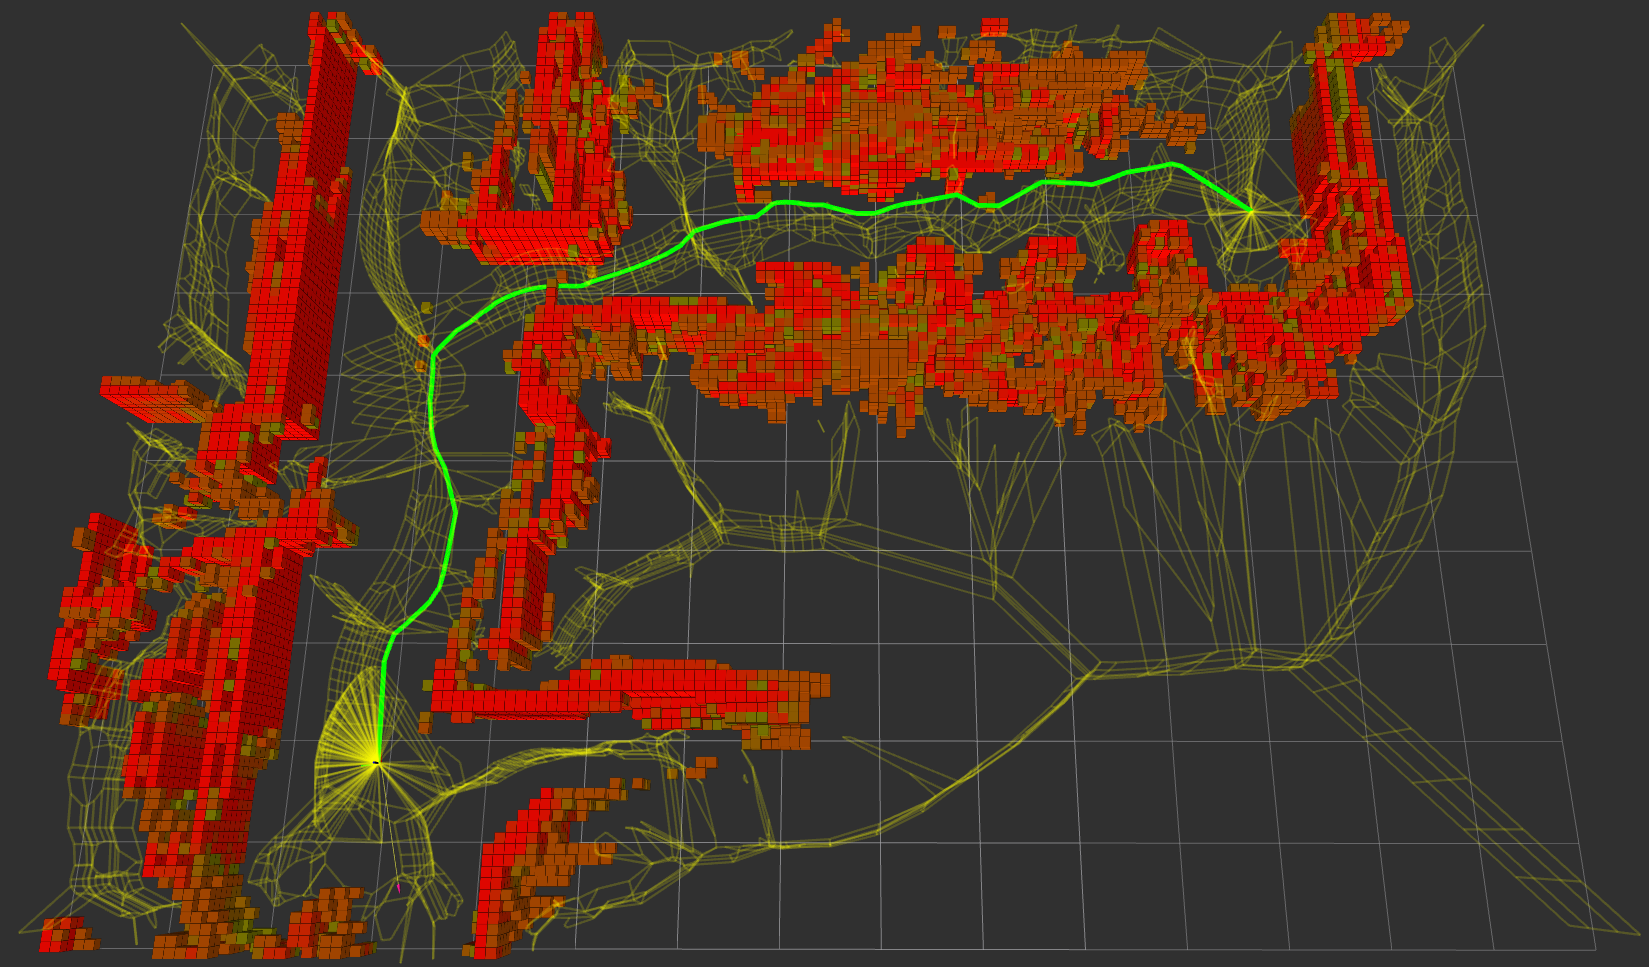
\includegraphics[width=.65\textwidth]{navigation_stack}
    \caption{Mapping and navigation algorithms execution.}
    \label{fig:navstack}
  \end{figure}
\end{frame}


% --- Section 6 ---
% Section 4 - Simultaneous Localization And Mapping
% Roberto Masocco <roberto.masocco@uniroma2.it>
% June 5, 2024

% ### Simultaneous Localization And Mapping ###
\section{Simultaneous Localization And Mapping}
\graphicspath{{figs/section4/}}

% --- Simultaneous Localization And Mapping ---
\begin{frame}{Simultaneous Localization And Mapping}{Definition}
	The \textbg{SLAM} problem is a \textbg{chicken-and-egg} problem: a robot must \textbg{localize itself} within an environment, while \textbg{mapping} it.\\
	\bigskip
	The ultimate goal of SLAM is to enable the robot to \textbg{navigate} within the environment, while \textbg{updating} the map as it moves.\\
	\bigskip
	The robot must be able to \textbg{efficiently} and \textbg{accurately} build a map of the environment, while \textbg{localizing itself} within it, with respect to either the origin of the map or the starting point of the robot itself (\emph{i.e.}, with either some or none \textbg{prior notion of the environment}).\\
	\bigskip
	To solve this problem, \textbg{sensor fusion} techniques are often employed, mixing data coming from \textbg{heterogeneous sensors} and accounting for \textbg{sensor faults}.\\
  \bigskip
  Typically, SLAM algorithms rely on recognizable \textbg{features} of the environment to build the map and detect motion.
\end{frame}
\begin{frame}{Simultaneous Localization And Mapping}{Loop closure}
  \begin{columns}
    \column{.5\textwidth}
    While a SLAM system builds a \textbg{map} of the environment, it can detect whether it is exploring a zone that it has \textbg{already visited}.\\
    \medskip
    When this happens, the system can \textbg{close the loop} by \textbg{matching} the current "view" with a \textbg{previous one}, thus \textbg{correcting} the map and the robot's pose.\\
    \medskip
    This process is called \textbg{loop closure} and is a key feature of SLAM algorithms.\\
    \medskip
    Loop \textbg{detection} and \textbg{closing} must also be performed in real time, as well as the subsequent \textbg{corrections}; efficient optimization algorithms and data structures are crucial.

    \column{.5\textwidth}
    \begin{figure}
      \centering
      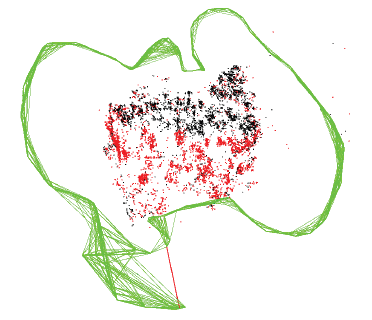
\includegraphics[width=.8\textwidth]{orbgraph}
      \caption{Loop closure of the ORB-SLAM2 algorithm.}
      \label{fig:loopclosure}
    \end{figure}
  \end{columns}
\end{frame}
\begin{frame}{Simultaneous Localization And Mapping}{Tools for the job}
  Sensors:
	\begin{itemize}
		\item \textbg{LIDARs} for direct environment mapping through depth information;
		\item \textbg{Cameras} to infer the environment structure through image processing;
		\item \textbg{IMUs} to account for the robot's motion and correct sampled data;
		\item \textbg{GNSS} to have a slow, but reliable global position estimate.
	\end{itemize}
  \medskip
  Plus all the \textbg{algorithms} and the \textbg{mathematical tools} we discussed in the context of \textbg{mapping}.
\end{frame}

% --- 2D SLAM ---
\begin{frame}{2D SLAM}{Cartographer}
  \begin{columns}
    \column{.55\textwidth}
    \textbg{Cartographer} is a \textbg{2D} SLAM algorithm developed by Google.\\
    \medskip
    Meant for \textbg{offline} floor plan generation, it has been ported in \textbg{ROS} for mobile robot navigation.\\
    \medskip
    It used \textbg{LiDAR} laser scans, corrected by \textbg{IMU} data, to build 2D \textbg{submaps} of the \textbg{surrounding} environment.\\
    \medskip
    Such maps are then used to \textbg{build and update} a \textbg{global map}, gluing submaps together and optimizing the result.\\
    \medskip
    Features are particular \textbg{environment structures} that are used to detect loop closures and estimate the robot's trajectory.

    \column{.45\textwidth}
    \begin{figure}
      \centering
      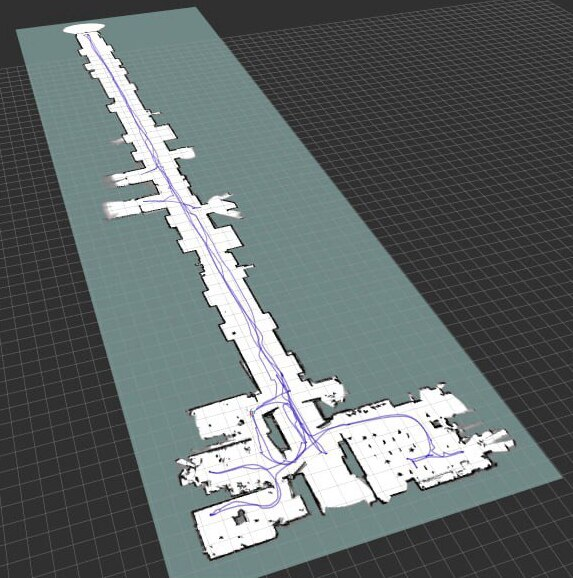
\includegraphics[width=.77\textwidth]{cartographer}
      \caption{Execution of the Cartographer SLAM algorithm.}
      \label{fig:cartographer}
    \end{figure}
  \end{columns}
\end{frame}

% --- Visual SLAM ---
\begin{frame}{Visual SLAM}{ORB-SLAM}
  \begin{columns}
    \column{.55\textwidth}
    \textbg{ORB-SLAM} is a \textbg{visual} SLAM algorithm that uses \textbg{monocular} or \textbg{stereo} cameras to build a map of the environment.\\
    \medskip
    It relies on \textbg{binary ORB features} to detect and match points in the environment, building a \textbg{covisibility graph} of \textbg{keyframes}: relevant views for pose estimation.\\
    \medskip
    The graph, and thus, the map and the camera pose estimate, are optimized with \textbg{bundle adjustment}.\\
    \medskip
    Latest versions also include \textbg{IMU} samples in the bundle adjustment cost function.

    \column{.45\textwidth}
		\begin{figure}
			\centering
			\movie[width=.85\textwidth, height=.6\textheight, poster, autostart, loop]{}{phd23_orb2-building-cut.mp4}
			\caption{ORB-SLAM2 algorithm execution on a ROS 2 dataset (bag).}
			\label{vid:building}
		\end{figure}
  \end{columns}
\end{frame}


\end{document}
